\section{Replacement Strategy}
\label{ch:replacement_strategy}

In the previous section, we introduce three semantics of permutation problems, three existing semantic models, MABMA. This section focuses on replacement strategy, give a brief introduction to the restricted tournament replacement (RTR) and incorporates these into the whole. This section defines three distance measures of RTR: edge distance, node distance and order distance, shows the effects of RTR on permutation problems and the essence of distance-measure choosing, proposes a method for choosing distance measure of RTR, improves reward policy of model adaptation, gives suggested setting of window size of RTR for permutation problems and shows the difference between original MABMA and MABMA with distance-measure choosing.




\subsection{Restricted Tournament Replacement}
The restricted tournament replacement (RTR) is a commonly used niching technique in the field of EDAs. RTR is also known as restricted tournament selection (RTS) which is first proposed in \citep{Harik1995}. RTR uses the tournament strategy to decide the part which get to move on to the next generation. We present the process of RTR in algorithm \ref{alg:RTR_algorithm}, where the $Distance$ function is usually the Hamming distance in binary problems. However, Hamming distance is not suitable for permutation problems. Thus, we define new distance for permutation problems by characteristics of permutation problems. The settings of window size $w$ are suggested in the following section.


\begin{algorithm}[htbp]
    \SetKwRepeat{doWhile}{do}{while}
    \KwIn{The original population $X=\lbrace x_1, x_2, ..., x_{n-1}\rbrace$\;
    The offspring population $Y$\;
    The window size $w$\; }
    \KwOut{The population $X$ of the next generation;}
    \For{ $y\in Y$ }
    {
        Choose a random subset $S =\lbrace s_0, s_1, ..., s_{w-1}\rbrace (0\leq s_i <n)$\;
        Find the $x_{s_i}$ in $\mathop{\argmin}_{{s_i} \in S} Distance(x_{s_i},y)$\;
        \If{$Fitness(y)>Fitness(x_{s_i})$}      {
        $x_{s_i} \leftarrow y$;
        }
        
    }
    return $X$\;
    \caption{The algorithm of RTR}
    \label{alg:RTR_algorithm}
\end{algorithm}


\subsection{Distance Metric}

This subsection defines three types of distance measures for RTR on permutation problems: edge distance, node distance and order distance. We define three distance measures by considering semantics of permutation problems.
\subsection*{Edge Distance}


An edge is connection between two nodes. The edge distance is calculated by different edge between two individuals. Let $D_{edge} (i,j)$ denote the edge distance between the two individuals $i$ and $j$, and \[ES_i=\lbrace\forall k(\pi_{(k\ mod\ L),i}, \pi_{(k+1\ mod\ L),i})\rbrace\mbox{ be an edge set of individual }i.\] Thus, $D_{edge} (i,j)$ is calculated as follows:\[D_{edge} (i,j)=L-\vert ES_i\cap ES_j\vert.\] For example, given two individuals $x=(1,2,3,4,5)$ and $y=(5,2,1,3,4)$, the edges $(1,5)$, $(2,3)$, $(1,3)$ and $(2,5)$ are not at the intersection of $ES_x$ and $ES_y$. The edge distance between $x$ and $y$ is $2$. 


\begin{figure}[htbp] 
        \centering
        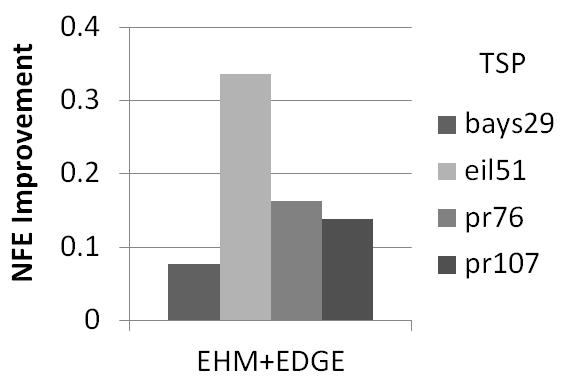
\includegraphics[width=0.5\textwidth]{EHM+edge.png}
        \caption{ Improvements in NFE of EHM with the edge distance } 
        \label{fig:ehbsa_imp}
\end{figure}

For investigating the efficiency of the edge distance, we test EHM and EHM+RTR which uses the edge distance on TSP with the minimum required population size which is the minimum size for solving the objective problem, maximum NFE $E_{max} = \ell\times 40000$ and the number of cut points which is 3, and repeat 20 times respectively. Figure \ref{fig:ehbsa_imp} shows NFE reduced by RTR with the edge distance. 
The results indicate that RTR with the edge distance is able to improve the performance of EHM on TSP. Besides, as the difficulty of permutation problem growing up, the improvement increases. By the way, the problem size of $pr76$ is larger than $eil51$, but the minimum required population size of $pr76$ is smaller than $eil51$. This means that $eil51$ is more difficult problem than $pr76$. 

\subsection*{Node Distance}
The node distance is calculated by each node at different position between two individuals. Let $D_{node} (i,j)$ denote the node distance between the two individuals $i$ and $j$. $D_{node} (i,j)$ is calculated as follows:\[D_{node} (i,j)=\sum_{k=0}^{ell-1} r_{i,j} (k), \]
where $r_{i,j} (k)$ is a function defined as \[r_{i,j} (k)=
\begin{cases}
1,  & \mbox{if }\pi_{k,i}\neq \pi_{k,j} \\
0, & \mbox{otherwise}
\end{cases}
.\] For example, given two individuals $x=(1,2,3,4,5)$ and $y=(5,2,1,3,4)$, the nodes $1$, $3$, $4$ and $5$ are not at the same position in both individuals. Thus, the node distance between $x$ and $y$ is $4$.



\begin{figure}[htbp] 
        \centering
        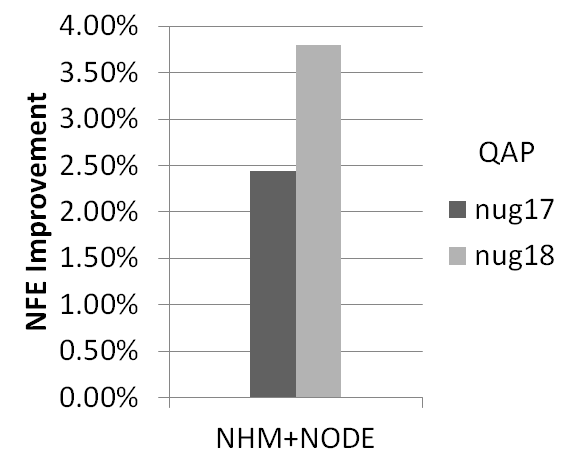
\includegraphics[width=0.5\textwidth]{NHM+node.png}
        \caption{ Improvements in NFE of NHM with the node distance } 
        \label{fig:nhbsa_imp}
\end{figure}


For investigating the efficiency of the node distance, we test NHM and NHM+RTR which uses the node distance on QAP with the minimum required population size, maximum NFE $E_{max} = \ell\times 40000$ and the number of cut points which is 3, and repeat 20 times respectively. Figure \ref{fig:ehbsa_imp} shows NFE reduced by RTR with the node distance. The results indicate that RTR with the node distance is able to improve the performance of NHM on QAP.



\subsection*{Order Distance}
The order distance is calculated by different orders of every node pair between two individuals. Let $D_{order} (i,j)$ represent the order distance between the two individuals $i$ and $j$, and \[OS_i=\lbrace\forall x,y(\pi_x^i,\pi_y^i)| x>y\rbrace\mbox{ be an order set of individual }i.\] The order distance $D_{order} (i,j)$ is calculated as follows:\[D_{order} (i,j)=\binom{\ell}{2}-\vert OS_i\cap OS_j\vert.\]
Consider an example of order distance, two individuals $x=(1,2,3,4,5)$ and $y=(5,2,1,3,4)$ are given, the orders $(1,2)$, $(1,5)$, $(2,5)$, $(3,5)$, $(4,5)$ are not at the intersection of $OS_x$ and $OS_y$. Thus, the order distance between $x$ and $y$ is $2$. 




\begin{figure}[htbp] 
        \centering
        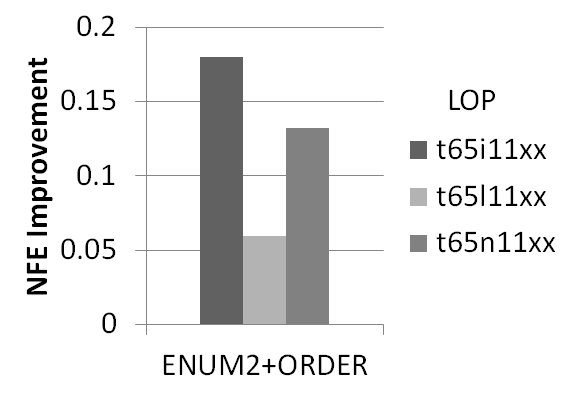
\includegraphics[width=0.5\textwidth]{ENUM2+ORDER.png}
        \caption{ Improvements in NFE of EHM+NHM with the order distance } 
        \label{fig:enum2_imp}
\end{figure}


For investigating the efficiency of the order distance, we test Enum2 and Enum2+RTR which uses the order distance on LOP with the minimum required population size and maximum NFE $E_{max} = \ell\times 40000$, and repeat 20 times respectively. In this experiment, we use the enumeration method to choose model. Figure \ref{fig:enum2_imp} shows NFE reduced by RTR with the order distance. The results indicate that RTR with the order distance is able to improve the performance of Enum2 on LOP. 


\subsection{Essence of Distance-measure Choosing}
This section shows the essence of distance-measure choosing. For the same reason of essence of model adaptation, the mechanism of distance-measure adaptation is necessary. 


For Investigating the essence of distance-measure choosing, we test EHM with the edge distance, EHM with the node distance, NHM with the edge distance and NHM with the edge distance on QAP and TSP. We perform independent 20 runs with maximum NFE $E_{max} = \ell \times 40000$ and the population size $N=\ell\times 2$ for each iteration. The results are shown in Figures \ref{fig:essence2}. As we can see, EHM+RTR with the edge distance outperforms EHM with the node distance, and NHM with the node distance outperforms NHM with the node distance. This means that RTR with the correct distance measure outperforms that with wrong distance measure but model choosing is more important than distance-measure choosing on permutation problems.

\begin{figure}[htbp] 
        \centering
        \begin{subfigure}{1\textwidth}
            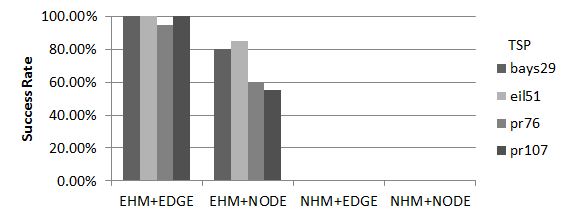
\includegraphics[width=\textwidth]{essenceTSP.png}
            \caption{  Success rates of the algorithms on TSP } 
        \end{subfigure}

        \begin{subfigure}{1\textwidth} 
            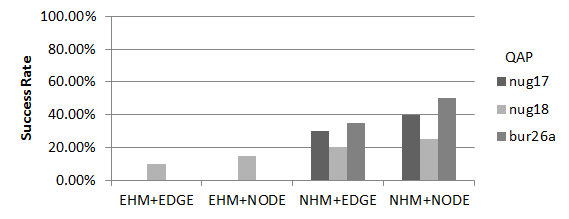
\includegraphics[width=\textwidth]{essenceQAP.png}
            \caption{ Success rates of the algorithms on QAP}
        \end{subfigure}
        
        \caption{ Results of EHM+EDGE, EHM+NODE, NHM+EDGE and NHM+NODE on TSP and QAP } 
        \label{fig:essence2}
\end{figure}


In another experiment, we choose the edge distance with the probability $p$ and choose the node distance with the probability $1-p$ at each generation, and use enumeration method to choose EHM or NHM. The probability $p$ starts from 0.0 to 1.0 and increases 0.1 by each iteration. the instances of LOP are used : $t65i11x$ and $t65n11x$ from LOLIB. We perform independent 10 runs with the maximum NFE $E_{max} = \ell \times 40000$ for each iteration. The results are shown in Figure \ref{fig:sweep_imp}. We can find that the best performance is not at maximum or minimum of $p$. This experiment indicates that mixing different distance measure can solve permutation problems more effectively.



\begin{figure}[htbp] 
        \centering
        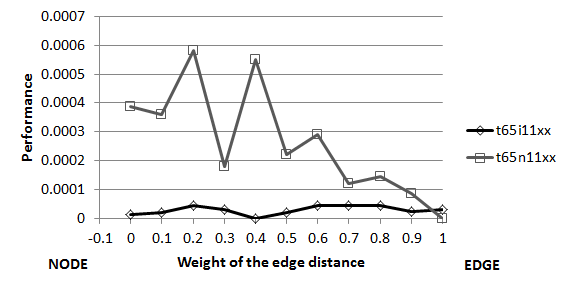
\includegraphics[width=0.9\textwidth]{essence.png}
        \caption{ Success rates of EHM+NHM with the sweeping probability choosing the node distance. } 
        \label{fig:sweep_imp}
\end{figure}


\subsection{Model-associated Method}
In this section, we introduce the model-associated method. The model-associated method is a method of distance-measure choosing. In each RTR, the model-associated method chooses the corresponding distance measure with the semantic model which selected on model-choosing phase. For example, let $MS=\langle m_1 , m_2, ..., m_{N_M}\rangle$ be an ordered set of semantic models and $DS=\langle d_1 , d_2, ..., d_{N_M}\rangle$ be an ordered set of distance measures, where ${N_M}$ is the number of models, $m_i$ represents the semantic model $i$ and $d_i$ denotes the corresponding distance measure of the semantic model $i$. Table \ref{tb:model_distance} shows the semantic models and their corresponding distance measures in our work.


\begin{table}[htbp]
    \centering
    \begin{tabular}{|l|l|}
    \hline
    \textbf{Semantic Models}       & \textbf{Corresponding Distance}  \\ \hline
    \textbf{NHM} & Node Distance    	 \\ \hline
    \textbf{EHM} & Edge Distance  	\\ \hline
    \textbf{PL} & Order Distance  	\\ \hline
  
    \end{tabular} 
    \caption{Semantic models and their corresponding distance measures}
    \label{tb:model_distance}
\end{table}

\begin{figure}[htbp] 
        \centering
        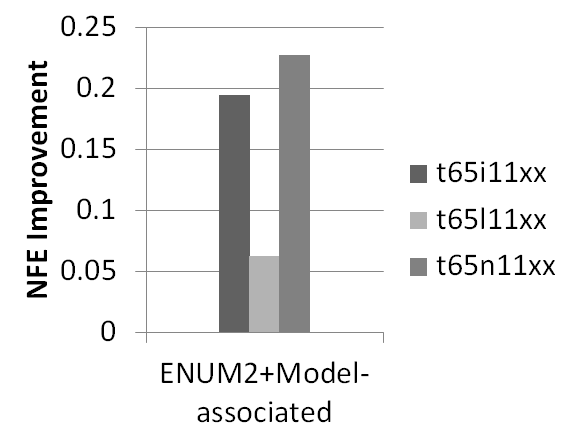
\includegraphics[width=0.5\textwidth]{ENUM2+model.png}
        \caption{ Improvements in NFE of RTR with the model-associated method on LOP } 
        \label{fig:enum2_model}
\end{figure}

To investigate the performance of the model-associated method, we test EHM+NHM and EHM+NHM with the model-associated method on LOP with the minimum required population size, maximum NFE $E_{max} = \ell\times 40000$ and the number of cut points which is 3, and repeat 20 times respectively. In this experiment, we use enumeration method to choose EHM or NHM. The results are shown in Figure \ref{fig:enum2_model}. The results shows that RTR with the model-associated method is able to improve the performance of EHM+NHM on LOP. Comparing with the experimental results of the order distance, the performance of RTR with the model-associated method is close to that with the order distance. 

\subsection*{Reward Policy}

Based on the assumption that the successes of the replacements with RTR keeps more information, we modify the reward policy of model adaptation. We change the reward policy $r$ from \[r=
\begin{cases}
1,  & \mbox{if the new individual is better than template~~~~~~~~~~~~~~~~~~~~ }\\
0, & \mbox{otherwise}
\end{cases}
\]to\[r=
\begin{cases}
1,  & \mbox{if the new individual is better than the one choosen by RTR}\\
0, & \mbox{otherwise.}
\end{cases}
\]
To investigate the performance of the new reward policy, we test MABMA with the model-associated method using the original reward policy and the new reward policy respectively. In this experiment, EHM and NHM are used, the instances of TSP are used: $bays29$, $eil51$, the population size $N$ is $\ell$ and maximum NFE $E_{max}$ is $\ell\times 40000$. We compare the usage of the correct semantic model--EHM at $3000$-th generation and the fitness on termination.  The results are shown in Table \ref{tb:reward}.  This experiment indicates that the new reward policy outperform the original reward policy.  As we can see, the usage of EHM with the new reward policy is higher than with the original reward policy at $3000$-th generation. EHM would keep higher usage for a long time until the successful replacement is hard for both semantic models. This is means that the semantic RTR is helpful for the model adaptation.

\begin{table}[htbp]
    \centering
    \begin{tabular}{|l|l|l|}
    \hline
    \textbf{Reward Policy}       &\textbf{Higher usage of EHM}       & \textbf{Achieving higher fitness}  \\ \hline
    \textbf{The original reward} & 21/50 & 14/50   	 \\ \hline
    \textbf{The modified reward} & 29/50 & 36/50	\\ \hline
    \end{tabular} 
    \caption{The result of comparing between the original reward and the modified reward on TSP}
    \label{tb:reward}
\end{table}
\subsection*{Window Size}

In this subsection, we investigate the window size of RTR on permutation problems. For this purpose, we test EHM with the edge distance, NHM with the node distance and PL with the order distance on the following instances:
\begin{itemize}
    \item TSP:$bays29$, $ berlin52$, $ ch130$, $ dantzig42$, $eil51$, $ eil76$, $eil101$, $ fri26$, $ gr17$, $gr24$, $ gr48$, $ gr96$, $ gr137$, $ hk48$, $ pr76$, $ pr107$, $pr124$, $ pr136$, $rat99$, $st70$, $swiss42$, 
    \item QAP:$bur26a$, $ bur26b$, $ bur26c$, $bur26d$, $ nug17$, $nug18$, $ nug20$, $ nug21$, $tai10a$, $tai10b$, $tai12a$, $tai12b$, $tai15a$, $tai15b$, $tai20a$, $tai25a$, $tai30a$, $tai35a$, $tai35b$, $tai40a$ and
    \item LOP:$t75i11xx$, $t65f11xx$, $ t65b11xx$, $ t65d11xx$, $ t65i11xx$, $t65l11xx$, $ t65n11xx$, $ t65w11xx$, $ t69r11xx$, $t70b11xx$, $ t70d11xx$, $ t70d11xxb$, $be75eec$, $ be75np$, $ be75oi$, $ tiw56n54$, $tiw56n58$, $ tiw56n66$, $stabu70$, $ stabu74$, $ usa70$
\end{itemize} 
, with the different window sizes, the population size $N=\ell$ and maximum NFE $E_{max}=\ell\times 5000$, the corresponding distance measures, and repeat three times respectively. In the experiments, we keep the template in the window of RTR at each generation. The performance measure employed in our study is the number of best rank which mean that the algorithm with the size has best performance of NFE and fitness.

\begin{figure}[htbp] 
        \centering
        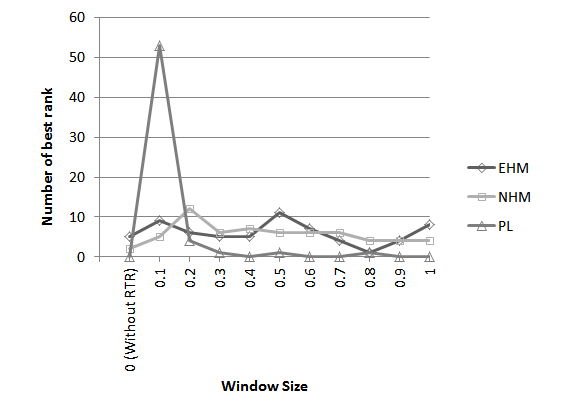
\includegraphics[width=1\textwidth]{window_size.png}
        \caption{ Rank results of EHM, NHM and PL with different window sizes } 
        \label{fig:w_size}
\end{figure}



The results are shown in Figure \ref{fig:w_size}. As we can see, the point of EHM with the window size $w=\ell\times 0.5$ overall has the lowest ARPD for all instances. The point of NHM with the window size $w=\ell\times 0.2$ overall has the lowest ARPD for all instances for NHM, and the point of PL with the window size $w=\ell\times 0.1$ overall has the lowest ARPD for all instances for PL. The point with window size $w=0$ is identical to the algorithm without RTR in our experiments. Finally, we give the suggested settings of the window size as follows:
\begin{itemize}
    \item the window size for EHM is $\ell\times 0.5$,
    \item the window size for NHM is $\ell\times 0.2$
    \item and the window size for PL is $\ell\times 0.1$.
\end{itemize}




In another experiment, we investigate whether the template should be included in the window of RTR. The results are shown in Figure \ref{fig:w_template}. The performance measure employed in our study is the average relative percentage deviation (ARPD):\[ARPD=\left|\left(\sum_{i=1}^{runs}\frac{Best-Result_i\times 100}{Best} \times \frac{1}{runs}\right)\right|\], where $Result_i$ is the best fitness found by the algorithm in the $i-th$ repetition, $Best$ is the fitness of the best known solution and $runs$ is 3 in this experiment. The performance of including template in the window outperforms. This is because of the information contained in template. The template is the lower bound of RTR.


\begin{figure}[htbp] 
        \centering
        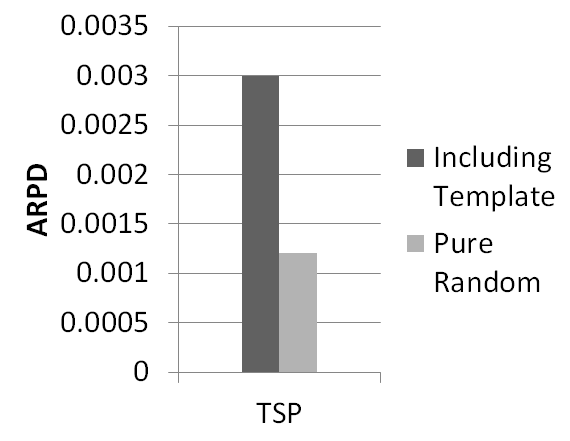
\includegraphics[width=0.5\textwidth]{include_template.png}
            \caption{ARPD results of the algorithm including the template in window and pure random picking} 
        \label{fig:w_template}
\end{figure}
\subsection{Empirical Study}
In this section, we investigate the performance of RTR with the model-associated method. For this purpose, we perform MABMA with the model-associated method and the original. The experimental settings are as follows:
\begin{itemize}
    \item repeat 20 times,
    \item EHM, NHM and PL are used,
    \item the number of cut points is 3 for template,
    \item maximum NFE $E_{max}$ is $\ell \times 40000$,
    \item the population size $N$ is $\ell \times 2$,
    \item the new reward policy is used,
    \item the window size is $\ell\times 0.5$ for EHM, $\ell\times 0.2$ for NHM and $\ell\times 0.1$ for PL,
    \item the benchmark instances of TSP :$bays29$, $eil51$, $pr76$, $kroA100$ and $pr107$ are used,
    \item the benchmark instances of QAP :$nug17$, $nug18$, $bur26a$, $ tai30b$ and $bur26b$ are used,
    \item the benchmark instances of LOP :$t65b11x$, $t65b11x$, $t65d11x$, $t65f11x$ and $t65n11x$ are used,
    \item the benchmark instances of CVRP $:A-n32-k5$, $A-n33-k5$, $A-n33-k6$, $A-n34-k5$ and $A-n36-k5$ are used
    \item and the benchmark instances of FSSP :$20\_5\_01\_ta001$, $20\_10\_01\_ta011$, $20\_20\_01\_ta021$, $50\_5\_01\_ta031$ and $50\_10\_01\_ta041$ are used.
\end{itemize}

Figure \ref{fig:arpdi} shows the ARPD results of MABMA and MABMA with the model-associated method. Comparing the performance of our proposed method with the original MABMA, the ARRD results of our proposed method are smaller than the ARRD results of original MABMA on each problem, in other words, MABMA with the model-associated method outperforms the original. This indicates that our proposed method is close to the best performing model with RTR and outperforms any single model without that in this work.

%Combining RTR, distance-measure choosing, the modified reward policy and the suggested window sizes, our proposed method is close to the  best performing model with RTR and outperforms any single model without that in this work. 
\begin{figure}[htbp] 
        \centering
        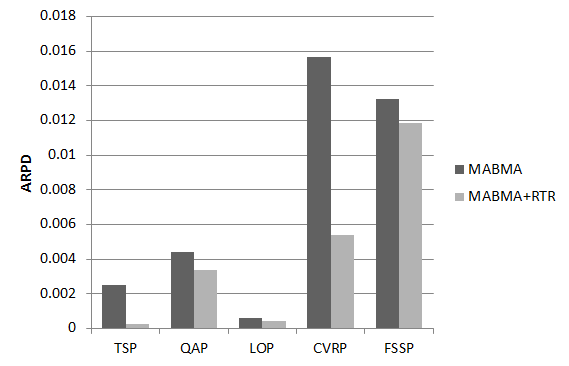
\includegraphics[width=1\textwidth]{arpdi.png}
        \caption{ ARPD results of MABMA and MABMA with the model-associated method on TSP, QAP, LOP, CVRP and FSSP. } 
        \label{fig:arpdi}
\end{figure}


